\documentclass[a4paper, 10pt]{scrartcl}
\usepackage[utf8]{inputenc}
\usepackage[ngerman]{babel}
\usepackage[T1]{fontenc}
\usepackage{helvet}
\usepackage{hyperref}
\usepackage{graphicx}

\title{Agiles und Statisches Modell im Vergleich}
\author{Mika Miosge}

\begin{document}
  \section{Die klassische bzw. statische Softwareentwicklung}
\subsection{Definition}
\begin{center}
\large{Klassische bzw. statische Softwareentwicklung ist eine Form der Softwareentwicklung bei welcher ein \glqq Software Development Life Cycle (SDLC)\grqq{} nach festem Ablaufplan umgestzt wird.\textsuperscript{[1]}} 
\end{center}
\subsection{Funktionsweise der klassichen bzw. statischen Softwareentwicklung}
Die klassiche Softwareentwicklung funktioniert nach dem Prinzip des SDLC. Dieser besteht aus 6 Phasen, welche alle nacheinander vom Entwicklungsteam abgearbeitet werden müssen.\textsuperscript{[1]} (siehe Abbildung 1)
\subsubsection{Analyse und Planung}
Die erste Phase dieses SDLC besteht aus der Analyse und Planung des Projektes. Sie ist gleichzeitig auch der wichtigste Entwicklungsabschnitt. Deshalb sollte dieser Schritt von den erfahrenen Teammitgliedern ausgeführt werden, um das bestmögliche Produkt zu erzeugen.\\  
In der ersten Phase der Entwicklung wird ein Projektplan aufgestellt, wie das Projekt uassehen soll und welche Schritte man durchläuft. Dabei kommt es natürlich auch auf das genaue Modell, welches zur Entwicklung benutzt wird an. Einige Besipiele dieser Modelle werden spätr erläutert. \\
Außerdm wird eine sogenannte Machbarkeitsstudie durchgeführt. Hierbei beschäftigt man sich damit, ob das Projekt auf wirtschaftlicher, bertrieblicher und technischer Sicht realisierbar ist. Das Ergebnis dieser Studie enthält verschiedene Softwareentwicklunsmethoden, welche dann nach gerinwgstem Implementierungsrisiko ausgewählt werden können.\\
Zudem wird in dieser Phase geplant, welche Inhalte für die Software unbedingt erforderlich sind. Außerdem werden Projektrisiken identifiziert um dagegen vorzugehen.\\
Ist dies geschafft, wird zur zweiten Phase übergegangen.
\subsubsection{Definition der erforderlichen Inhalte}
Im ersten Schritt wurden bereits die erforderlichen Inhalte der Software klar definiert und dokumentiert. In Rücksprache mit dem Kunden, werden diese dann gegebenfalls überarbeitet.\\
Die festgelegten Ziele werden in einer \glqq Software Requirement Specification (SRS)\grqq{} festegehalten. Die SRS ist dann eine Auflistung aller erforderlichen Inhalte der Software.\\
Danach geht es in der dritten Phase mit dem Projektaufbau weiter.
\subsubsection{Projektarchitektur}
In der dritten Phase des SDLC, entwickeln die Developer das Design bzw. die Architektur des Produktes. Dabei arbeiten sie mehrere Aufbaumöglichkeoten aus. Diese Möglichkeiten werden dann von allen interessierten Gruppen eingesehen und danach die Entscheidung für eine Variante gefällt. Die Entscheidung durch Abwägen bestimmter Kriterien, wie zum Beipsiel Risiko, Produktrobusheit, Designmethode, Budget, Dauer, etc., getroffen. \\
Am Ende dieser Phase, ist der Aufbau des Produktes klar definiert und man kann zum Programmieren übergehen.
\subsubsection{Produktimplemetierung}
In der vierten Phase startet die Produktentwicklung. Das bedeutet, dass nun der Code geschrieben wird. Dabei wird sich an das Prinzip, welches in der dritten Phase, Projektarchitektur, festgelegt wurde, gehalten. Dabei muss sich zwischen verschieden Modellen und auch verschiedenen Programmiersprachen, zum Beispiel Java oder Phython geschrieben werden. Dabei werden diese nach der Software, welche hergestellt werden soll, ausgewählt.\\
Nachdem die Software programmiert wurde, muss sie in der nächtsten Phase getestet werden.
\subsubsection{Testen des Produkts}
In dieser Phase werden Fehler im Produkt von Testern getestet. Fehler die auftreten werden gemeldet, dann von den Programmierern verfolgt und später behoben. \\ 
Diese Phase ist erfolgt eigentlich auch schon in den anderen Phasen der Entwicklung, da es gerade bei moderneren Produkten schon während der Entwicklung getestet wird.\\
Wenn alle Fehler behoben wurden, kann das Projekt veröffentlicht werden.
\subsubsection{Veröffentlichung und Überareitung}
Wenn all diese Schritte abgearbeitet wurden, kann das Produkt erst einmal auf einem Teil des Marktes veröfftlicht werden. Dann wird das Produkt unter realen Marktbedingungen getestet und Feedback eingeholt.\\
Je nachdem, wie dieses Feedback ausfällt, gibt es mehrere Möglichkeiten. 
\begin{itemize}
\item Wenn keine Fehler gefunden werden, kann das Produkt gleich auf dem ganzen Markt veröffentlicht werden.
\item Wenn Fehler gefunden werden, wird das Produkt überarbeitet und die Fehler behoben und mögliche Verbesserungen eingebaut. Danach wird das Produkt global gelaucht.
\end{itemize}
Werden nach der Veröffentlichung noch Probleme festgestellt, werden diese mit Updates behoben.

\begin{figure}
\begin{center}
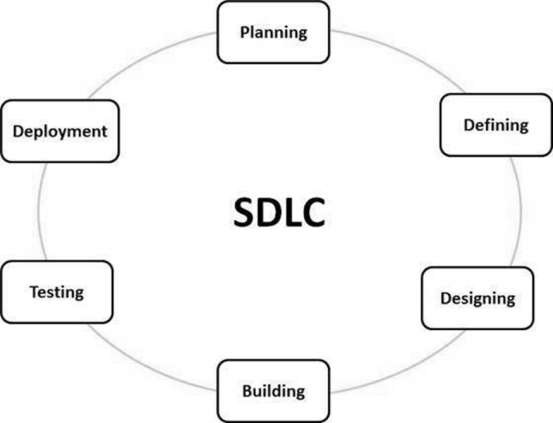
\includegraphics[width=10cm]{sdlc.jpg}
\caption{Abbildung 1: Der SDLC}
\end{center}
\end{figure}


\newpage
\section{Die Agile Softwareentwicklung}
\subsection{Definition}
\begin{center}
\large{\glqq{} Agile Softwareentwicklung ist eine Entwicklungsmethode die schnell auf veränderte Anforderungen reagieren kann, da die Entwicklung in vielen kleinen und abgeschlossen Zyklen abläuft und eine erhöhte Kommunikation zwischen den Entwicklern stattfindet.\grqq{}}\textsuperscript{[1]} \\
\end{center}

\subsection{Leitsätze der Agilen Softwareentwicklung}
Die Leitsätze des Agiles Modells wurden von 11 Softwareentwicklern, unter der \\Führung von Kent Beck im \glqq{}Manifest für Agile Softwareentwicklung\grqq{} festgehalten. Es gibt vier wesentliche Leitsätze der Agilen Softwareentwicklung, welche sie von \\anderen Softwareentwicklungsmodellen abgrenzt:
\begin{itemize}
\item \glqq{}\textbf{Individuen und Interaktionen} mehr als Prozesse und Werkzeuge\grqq{} \textsuperscript{[2]} 
\item \glqq{}\textbf{Funktionierende Software} mehr als umfassende Dokumentation\grqq{} \textsuperscript{[2]}
\item \glqq{}\textbf{Zusammenarbeit mit dem Kunden} mehr als umfassende Vertragsverhandlungen\grqq{} \textsuperscript{[2]}
\item \glqq{}\textbf{Reagieren auf Veränderung} mehr als das Verfolgen eines Plans\grqq{} \textsuperscript{[2]}
\end{itemize}
Angemerkt sei, dass die Entwickler des Agilen Modelles keinesfalls die Werte auf der rechten Seite als unwichtig betrachten, sondern die Werte auf der linken Seite als wichtiger im Prozess der Softwareentwicklung einschätzen.\\
Außerdem gibt es im Maifest eine Erweiterung der auf 12 Prinzipien, welche die oben genannten Prizipien näher erklären.\textsuperscript{[2]} 
\subsection{Prinzipien der Agilen Softwareentwicklung\textsuperscript{[2]}}
Ein Prinzip des Agilen Modells, dass die Menschen, welche an der Entwicklung beteiligt sind miteinander interagieren.\\\\
Im Agilen Modell ist es wichtig, dass die Entwickler dem Kunden oft ihr Zwischenergebnis schicken, um den Kunden zufrieden zu stellen.\\\\
Dazu gehört die enge Zusammenarbeit zwischen Fachexperten und die Softwareentwickler sollen währendes Projektes täglich miteinander arbeiten.\\\\
Die Entwickler sollen Kunden alle Anforderungsänderungen erfüllen, um dem Kunden einen Wettbewerbsvorteil verschaffen zu können.\\\\
Die Entwickler sollen dem Kunden funktionierende Software innerhalb eines bestimmten Zeitraumes (einige Wochen oder Monate, aber schnellstmöglich) liefern, damit der Kunde den Fortschritt sehen kann.\\\\
Zudem sollte auf motivierte Individuen vertraut werden. Es sollte ihnen die Ünterstützung gewährleistet werden, damit sie die Aufgabe erledigen können. Das Wichtigste ist das Vertrauen in die Individuen, dass sie die Aufgabe bewältigen können.\\\\
Um im Entwicklungsteam Informationen auszutauschen, ist es die beste Methode dies im Gespräch zu erledigen.\\\\
Die Entwickler, Auftraggeber und die Benutzer sollen ein gleichmäßiges Tempo auf unbegrenzte Zeit halten können, um nachhaltige Entwicklung zu fördern.\\\\
Ständige Priorität sollten technische Exzellenz und gutes Design haben, um Agilität zu fördern.\\\\
Einfachheut ist im Agilen Modell sehr wichtig und wird als \glqq{}die Kunst, die Menge nicht
getaner Arbeit zu maximieren\grqq{}\textsuperscript{[2]} verstanden.\\\\
Die besten Ergebnisse mit diesem Modell können durch selbstorganisierte Teams erzielt werden.\\\\
Das gesamte Team soll in regelmäßigen Abständen selbst reflektieren, wann es seine Effektivität verbessern kann.
\subsection{Methoden, die sich für Agile Softwareentwicklung eignen}
Wie oben schon erwähnt, liegt der Fokus der Agilen Softwareentwicklung mehr Fokus auf den Entwicklern und deren Interaktion liegt, als auf den Werkzeugen, welche zur Programmierung verwendet werden. So kommt es, dass sich Methoden entwicklet haben, welche sich besonders gut für Agile Softwareentwicklung eignen.\\
Dazu wurde zum Beispiel die Methode der Paarprogrammierungn(auch \glqq Pair Programming\grqq genannt) entwickelt. Dabei geht es darum, dass \glqq zwei Entwickler an einem Rechner, um gemeinsam eine Aufgabe zu lösen.\grqq \textsuperscript{[3]}\\ Dabei soll die Methode \glqq die Qualität des Codes steigern, Wissen gleichmäßig verteilen und langfristig die Kommunikation und Produktivität im Team steigern.\grqq \textsuperscript{[3]}\\ Pair Programming funktioniert mit zwei Personen. Eine Person übernimmt die Rolle des Piloten. Dieser bedient den Computer und schreibt den Code. Die andere Person ist der Navigator. Dieser \glqq gibt Feedback zum aktuellen Code und denkt darüber nach, ob der Ansatz noch weiter verbessert werden kann\grqq \textsuperscript{[3]}. Außerdem hat der Navigator den Überblick über das ganze Projekt, dagegen konzentriert sich der Pilot mehr auf den aktuellen Abschnitt des Codes.\\Zudem bietet es sich bei dieser Methode an, die Rollen regelmäßig zu tauschen um eine gute Zusammenarbeit zu ermöglichen.\\Pair Programming ist bestens für die Agile Softwareentwicklung geeignet, da die Individuen, also die Entwickler im ständigen Austausch sind, somit die Kommunikation erhöht wird und auch die Arbeisergbnisse langfristig besser ausfallen.\ 

\subsection{Ziele bzw. Vorteile der Agilen Softwareentwicklung}
Aus den bereits aufgezeigten Prinzipien und Leitsätzen der Agilen Softwareentwicklung, kann man nun die Ziele  auch die damit verbunden Vorteile ableiten. \\
Schon die Prinzipien, die im \glqq{}Agilen Manifest\grqq{} niedergeschrieben wurden, geben Aufschluss darüber, was die Entwickler, welche dieses Modell der Softwareentwicklung nutzen, hinaus wollen.\\ Es wird Wert auf \glqq{}Individuen und Interaktionen, Funktionierende Software, Zusammenarbeit mit dem Kunden und das Reagieren auf Veränderung\grqq{} gelegt. Wie man erkennen kann, liegt der Fokus der Softwareentwicklung eher auf den Menschen, welche am Prozess der Entwicklung teilnehmen. So steht zum Beispiel der Kunde mit seine Wünschen im Vordergrund. Deshalb ist das Modell so ausgelegt, dass die Entwickler schnell auf Kundenwünsche bzw. -anregungen reagieren können.\\ Zudem werden auch die Entwickler mehr berücksichtigt und es werden auch spezielle Arbeitsmethoden angewendet (siehe oben)\\Außerdem empfinden die Nutzer der Agilen Softwareentwicklung die akribische Dokumentation des Schaffensprozesses als Behinderung der Arbeit und bauen lieber auf \glqq funktionierende Software\grqq. \\ 


\section{Quellen}
\subsection{Textquellen}
\begin{itemize}
\item[(1)] Stoica, Marian; Mireca, Marinela; Ghilic-Micu, Bogdan: Software Development: Agile vs. Traditional. In: \url{http://www.revistaie.ase.ro/content/68/06%20-%20Stoica,%20Mircea,%20Ghilic.pdf}
\item[(2)] \url{https://www.gruenderszene.de/lexikon/begriffe/agile-softwareentwicklung?interstitial_click}
\item[(2)] Beck, Kent: Manifesto for Agile Software Development. In: \url{https://pdfs.semanticscholar.org/213f/5fda7325903f1390bf84520c135a2fcd8e38.pdf?_ga=2.190010402.841701991.1580237983-73606039.1579679479} [zuletzt überprüft am 28.01.2019]
\item[(3)] Augsten, Stephan: Was ist Pair Programming?. In: \url{https://www.dev-insider.de/was-ist-pair-programming-a-788269/} [zuletzt überprüft am 22.01.2019]
\end{itemize}
\subsection{Bildquellen}
\url{http://www.tutorialspoint.com/sdlc/sdlc_overview.htm}
\end{document}



